\chapter{Prezentacja aplikacji oraz testy}
\section{Przedstawienie wyglądu aplikacji}
Użytkownik przechodząc pod adres \enquote{decisontree.pl} w przeglądarce zostanie przekierowany na stronę główną projektu (Rys. \ref{rys7_home_page} ). Zobaczy tam krótki opis czego dotyczy aplikacja. W celu korzystania z systemu wymagana jest autoryzacja użytkownika. Osoba nowa może założyć konto przy pomocy formularza rejestracji (Rys. \ref{rys8_registery_form}). Wypełniając pola użytkownik musi zaakceptować pole \textit{recaptcha}, pełniącą role zabezpieczenie przed botami grasującymi w internecie. Po zatwierdzeniu formularza osoba zostanie automatycznie zalogowana. Użytkownicy, którzy już posiadają konto w aplikacji mogą skorzystać z pola logowania przedstawionego na Rys. \ref{rys9_login_form}.

\begin{figure}[htb]
	\centering
	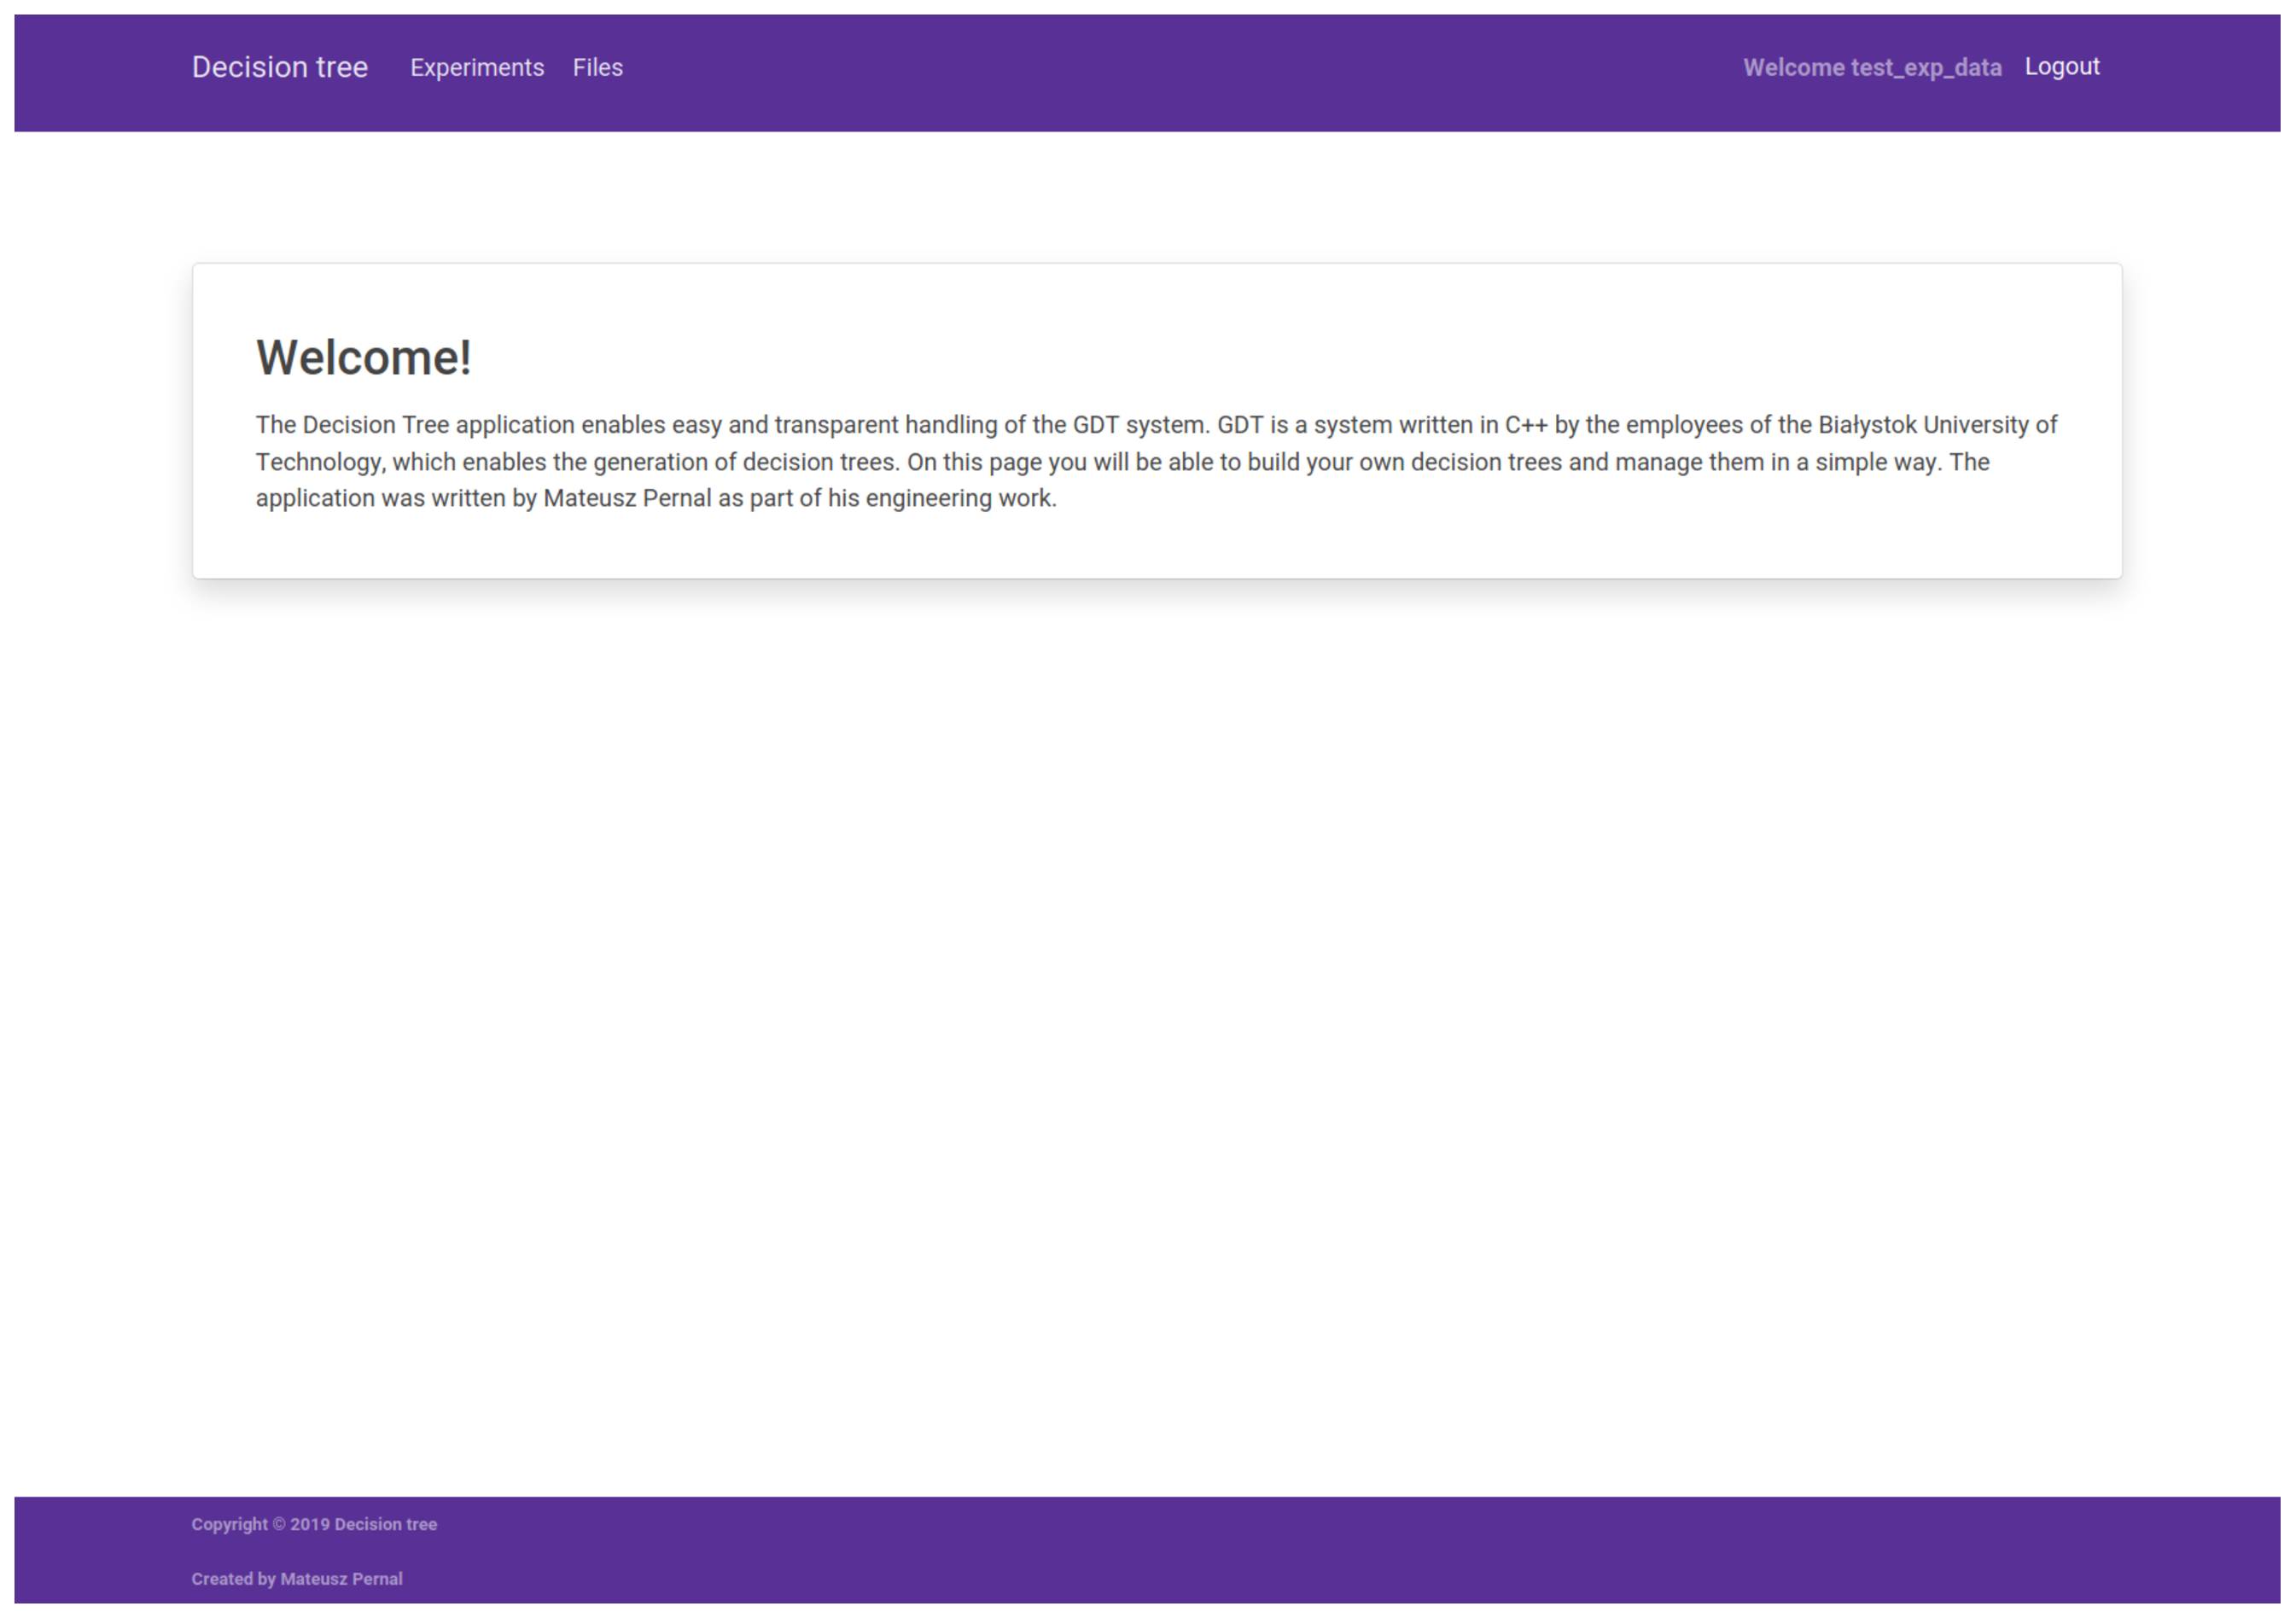
\includegraphics[width=15cm]{grafika/home_page.eps}
	\caption{Strona główna aplikacji.}
	\label{rys7_home_page}
\end{figure}

\begin{figure}[htb]
	\centering
	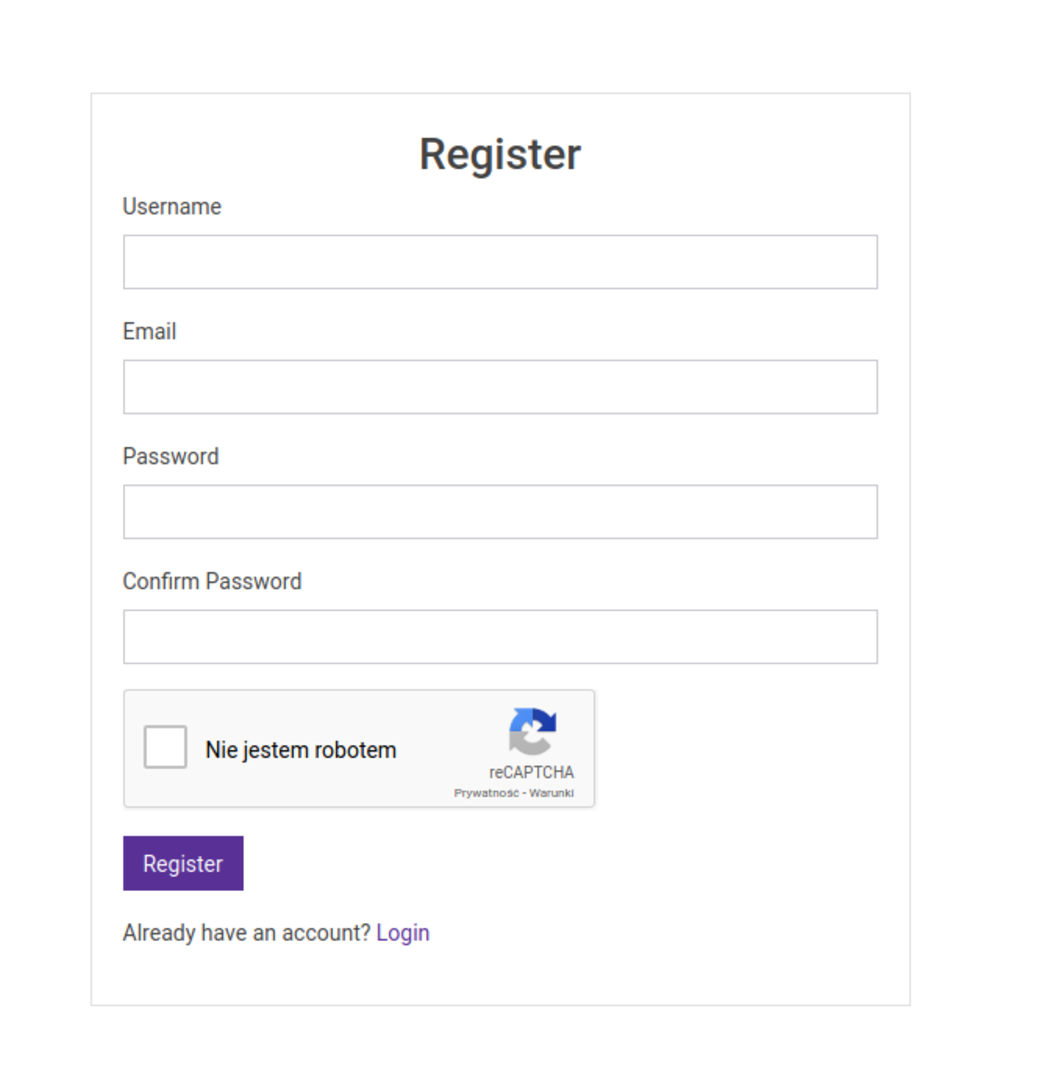
\includegraphics[width=11cm]{grafika/registery_form.eps}
	\caption{Formularz rejestracji nowego konta.}
	\label{rys8_registery_form}
\end{figure}

\begin{figure}[htb]
	\centering
	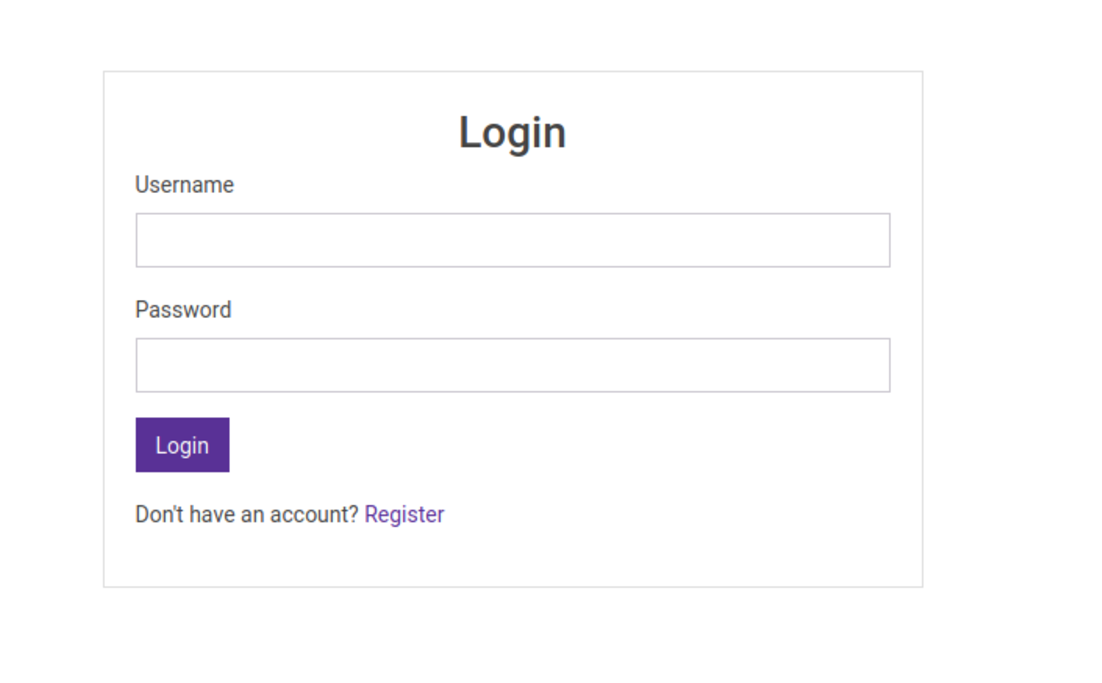
\includegraphics[width=11cm]{grafika/login_form.eps}
	\caption{Formularz logowania.}
	\label{rys9_login_form}
\end{figure}

Uwierzytelniony użytkownik w zależności od nadanych mu uprawnień będzie miał możliwe do wykonania inne akcje. 
Funkcjonalności do których nie będzie miał dostępu nie będą wyświetlane w interfejsie graficznym, na przykład mając uprawnienia z poziomu \enquote{1\_default} na pasku nawigacji nie będzie zakładki \enquote{Files}. Widok przedstawiający wygląd strony dla użytkownika ze wszystkimi prawami został pokazany na Rys. \ref{rys7_home_page}. Przechodząc do zakładki \enquote{Experiments} zostanie wyświetlona lista wszystkich eksperymentów wraz z przyciskiem do tworzenia nowego doświadczenia lub podglądem już istniejącego (Rys. \ref{rys10_experiment_table}). 
\begin{figure}[htb]
	\centering
	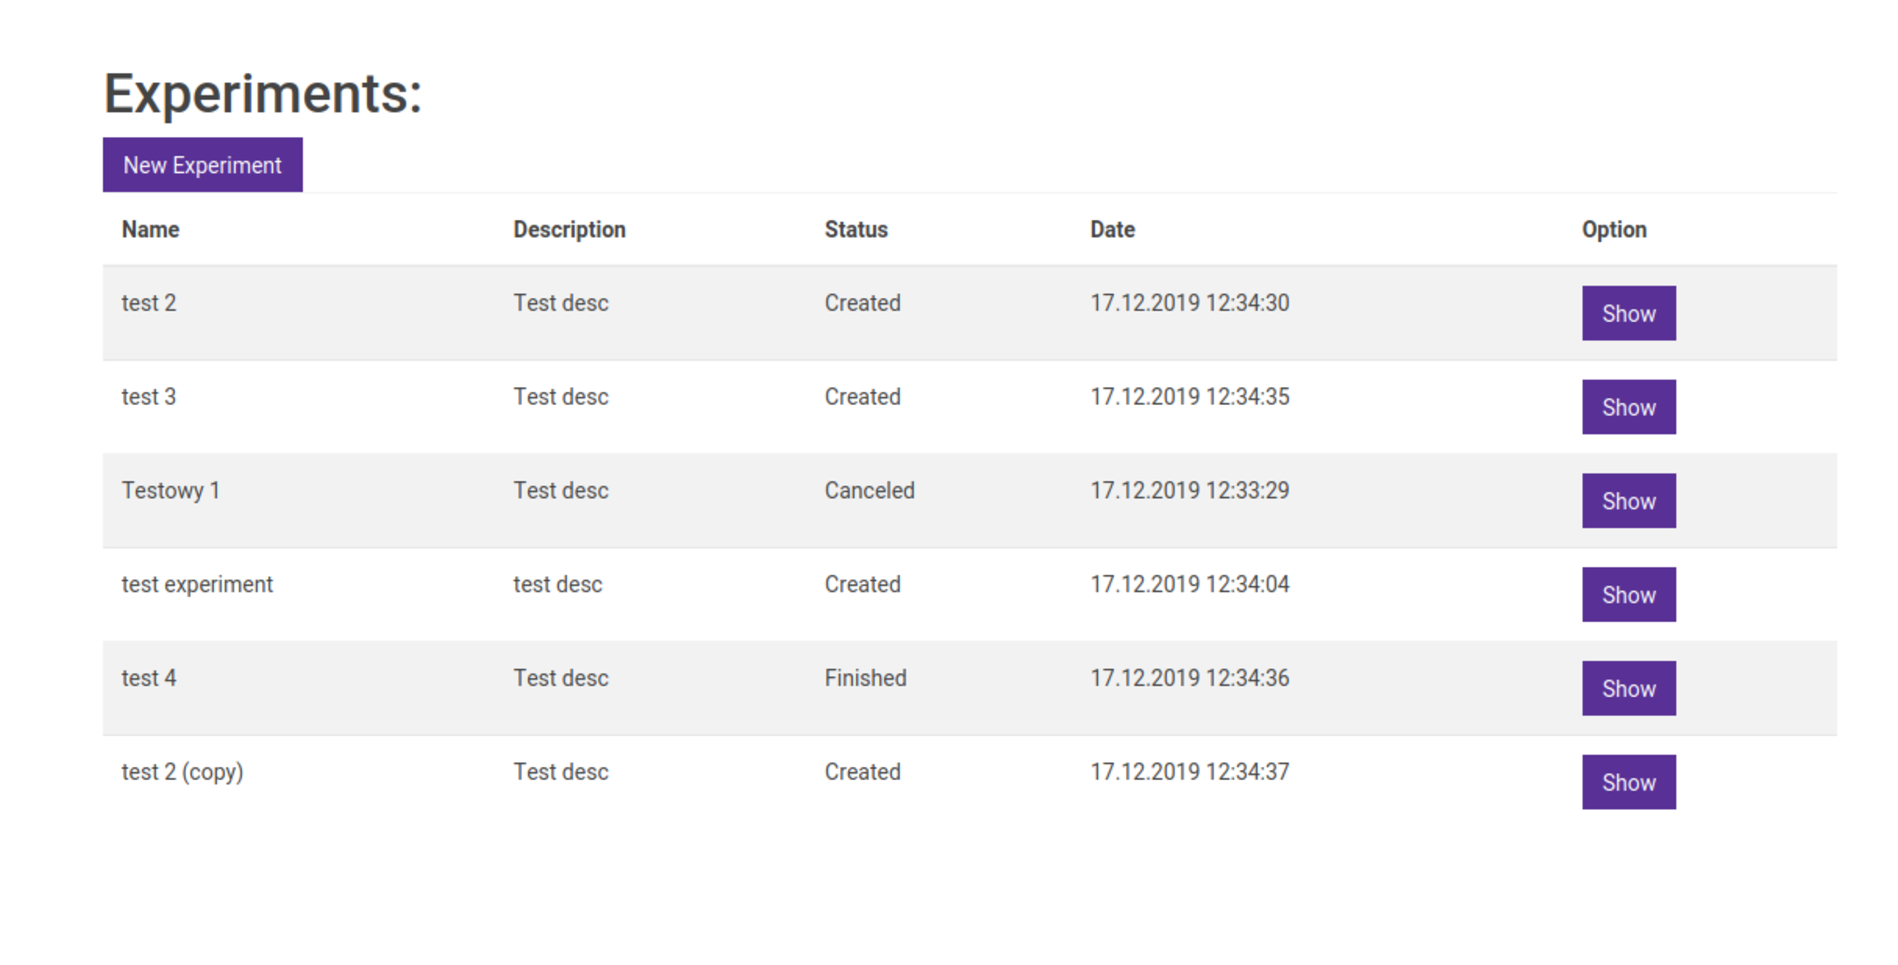
\includegraphics[width=15cm]{grafika/experiment_table.eps}
	\caption{Widok listy eksperymentów.}
	\label{rys10_experiment_table}
\end{figure}

\begin{figure}[htb]
	\centering
	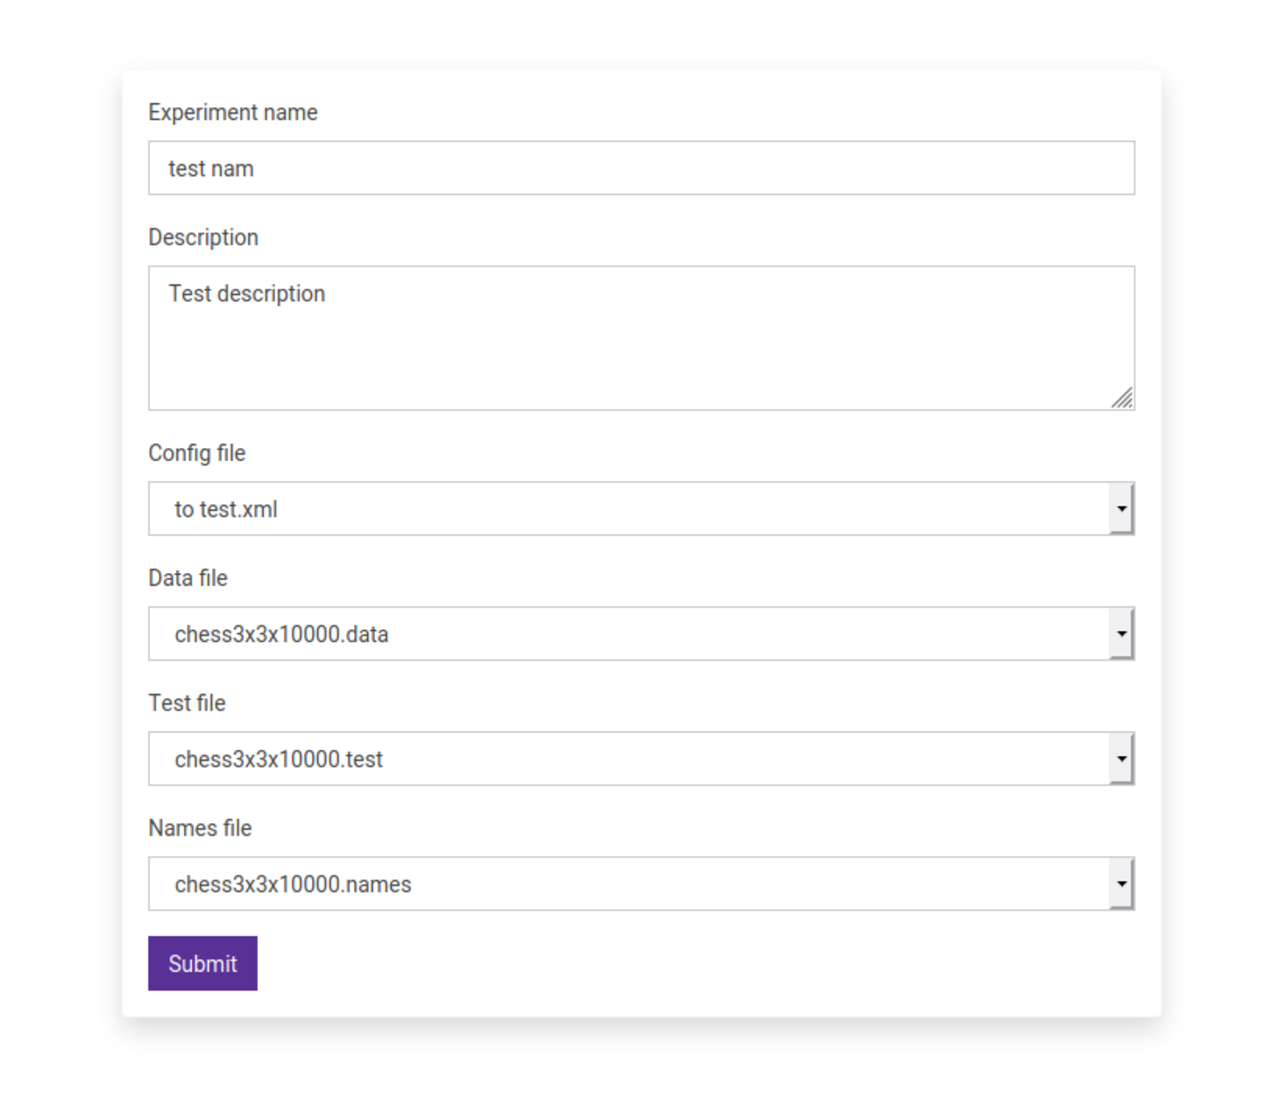
\includegraphics[height=9cm]{grafika/experiment_form.eps}
	\caption{Formularz tworzenia nowego eksperymentu}
	\label{rys11_experiment_form}
\end{figure}

Kolejnym elementem na pasku nawigacji jest odnośnik do strony zarządzania plikami użytkownika. Na tym widoku znajduję się drop zone umożliwiający wrzucanie plików niezbędnych do przeprowadzenia doświadczenia(Rys.\ref{rys17_file_page}). W dowolnym momencie osoba używająca aplikacji ma opcję zmiany nazwy((Rys.\ref{rys19_edit_name})), usunięcia oraz pobrania dowolnego pliku . Podczas próby uploadu pliku o rozszerzeniu innym niż tych co znajdują się na liście dozwolonych, dla użytkownika pojawi się alert błędu. Dodatkową funkcjonalnością dostępną na tej stronie jest przycisk kierujący do formularza tworzenia nowej konfiguracji. Formularz zawiera podstawowe pola, które są uzupełnione parametrami domyślnymi (Rys. \ref{rys18_config_form}). Stanowi to ułatwienie dla nowych użytkowników, którzy chcieliby zrobić swój pierwszy eksperyment bez zagłębiania się w zaawansowane zagadnienia.


\begin{figure}[htb]
	\centering
	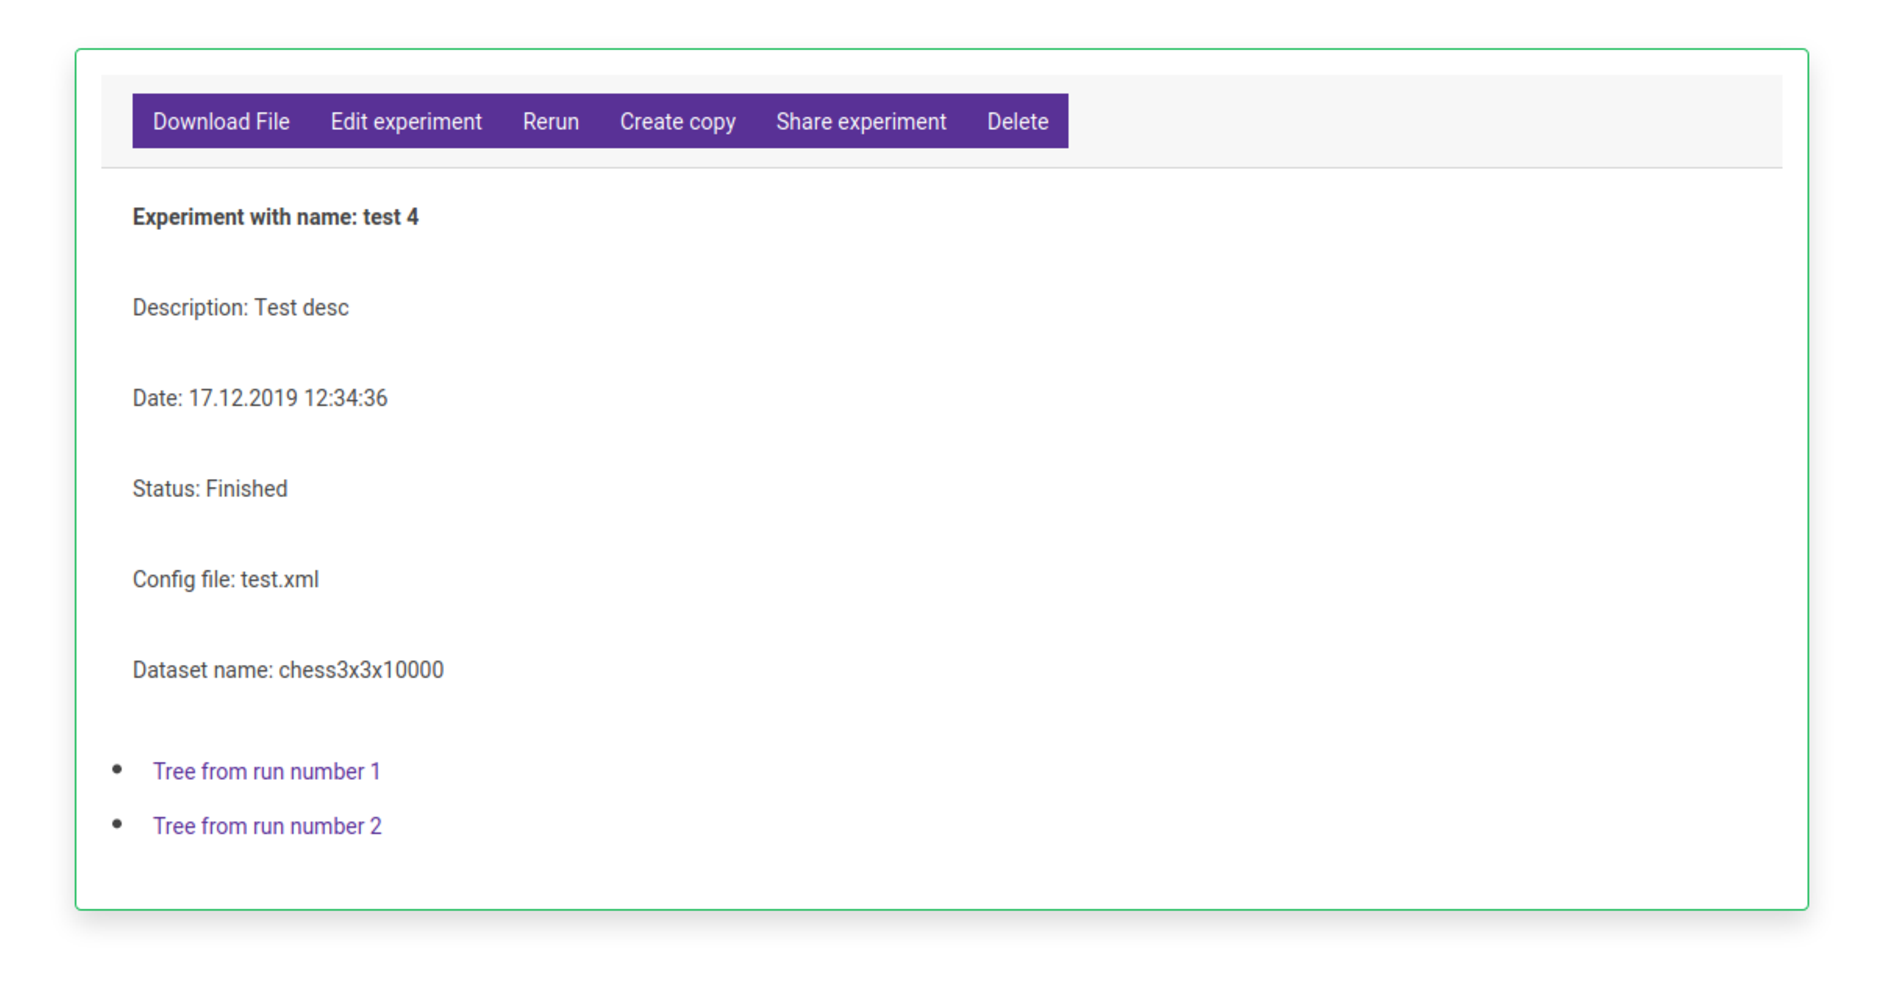
\includegraphics[width=15cm]{grafika/details_page.eps}
	\caption{Strona przedstawiający szczegóły eksperymentu.}
	\label{rys12_details_page}
\end{figure}

\begin{figure}[htb]
	\centering
	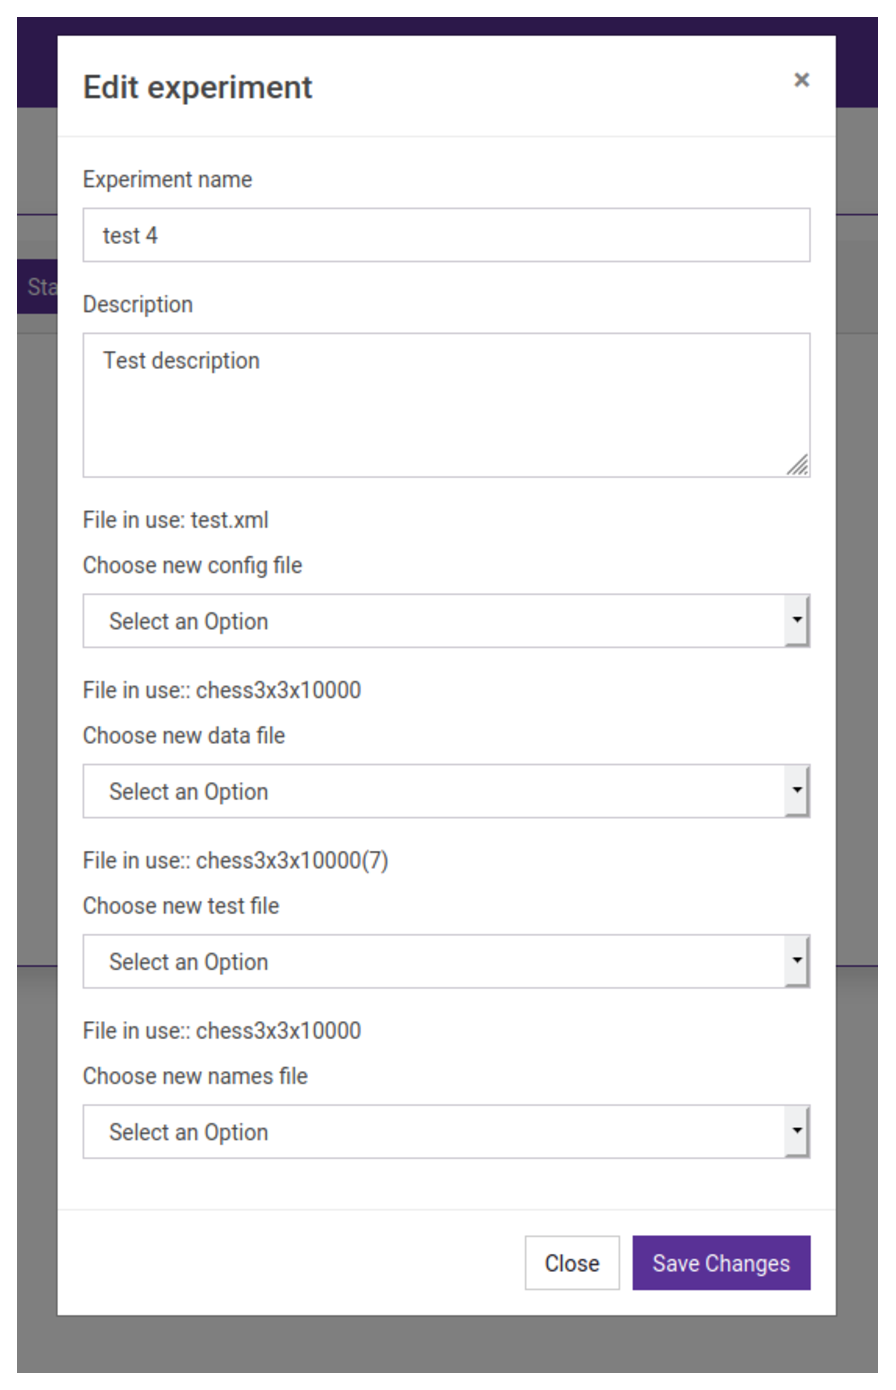
\includegraphics[height=11cm]{grafika/edit_experiment.eps}
	\caption{Formularz edycji eksperymentu.}
	\label{rys13_edit_experiment}
\end{figure}

\begin{figure}[htb]
	\centering
	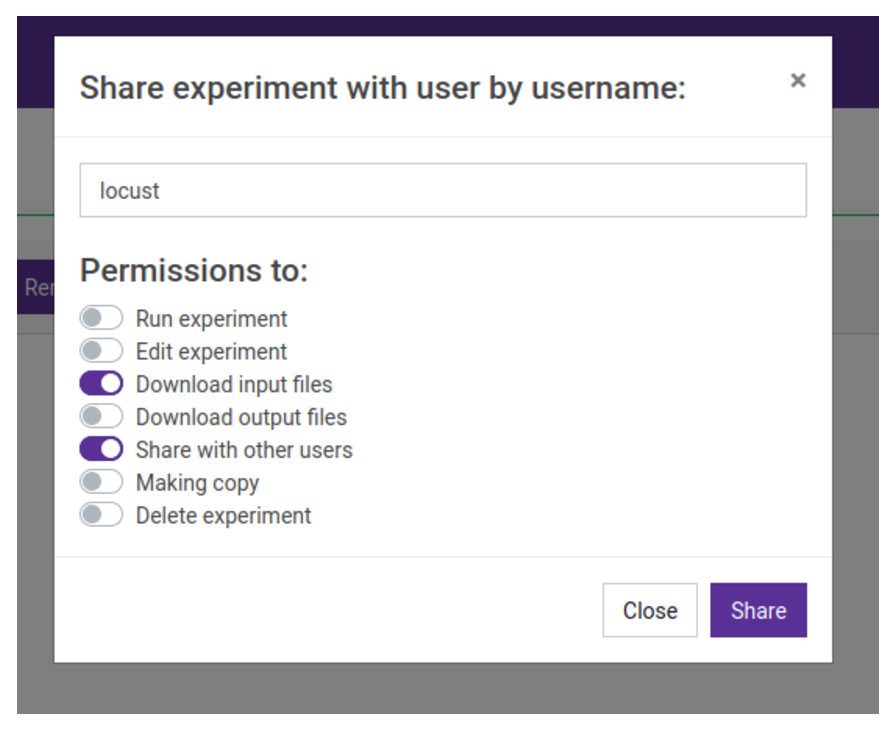
\includegraphics[width=11cm]{grafika/share_form.eps}
	\caption{Formularz udostępniania eksperymentu.}
	\label{rys14_share_form}
\end{figure}

Proces tworzenia nowego eksperymentu rozpoczyna się od wypełnienia formularza informacjami oraz wybraniu plików (Rys. \ref{rys11_experiment_form}). W przypadku zostawienia, któreś wartości pustej zostanie wyświetlony komunikat o błędzie. Jeżeli jednak wszystkie pola będą wypełnione, po zatwierdzeniu wyświetli się alert o sukcesie oraz nastąpi przekierowanie do listy eksperymentów. Nowo stworzone doświadczenia na liście posiadają status \enquote{Created}. Klikając w przycisk \enquote{Show} użytkownik może wyświetlić szczegóły eksperymentu, wraz z paskiem akcji możliwych do wykonania na nim. Po uruchomieniu doświadczenie trafia do kolejki i przyjmuje status \enquote{In queue}. Natomiast zaraz po zaczęciu obliczeń przechodzi w wartość \enquote{Running}, pozwala on na podejrzenie aktualnego postępu zadania w karcie szczegółów eksperymentu (Rys. \ref{rys15_progress_bar}. W dowolnym czasie trwania obliczeń pod doświadczenie wysłać sygnał przerwania, wtedy status zmieni się na \enquote{Cancel}. Kiedy podczas uruchomienia wystąpi błąd oznaczenie ustawi się na \enquote{Error}. W pełni ukończony eksperyment otrzymuje status \enquote{Finished}, a w widoku szczegółów pojawią się odnośniki do powstałych drzew (Rys.\ref{rys12_details_page}). W zależności od stanu doświadczenia ramka karty przyjmie inne kolory. Przechodząc do widoku z wynikami otrzymamy tabele ze statystykami takimi jak rozmiar drzewa, czas wykonania, rezultaty oraz ilość danych treningowych i testowych. Graf drzewa jest w pełni skalowalny przy pomocy kółka myszki, a poszczególne węzły można zwinąć. Dodatkową opcją jest możliwość wydrukowania schematu.




\begin{figure}[htb]
	\centering
	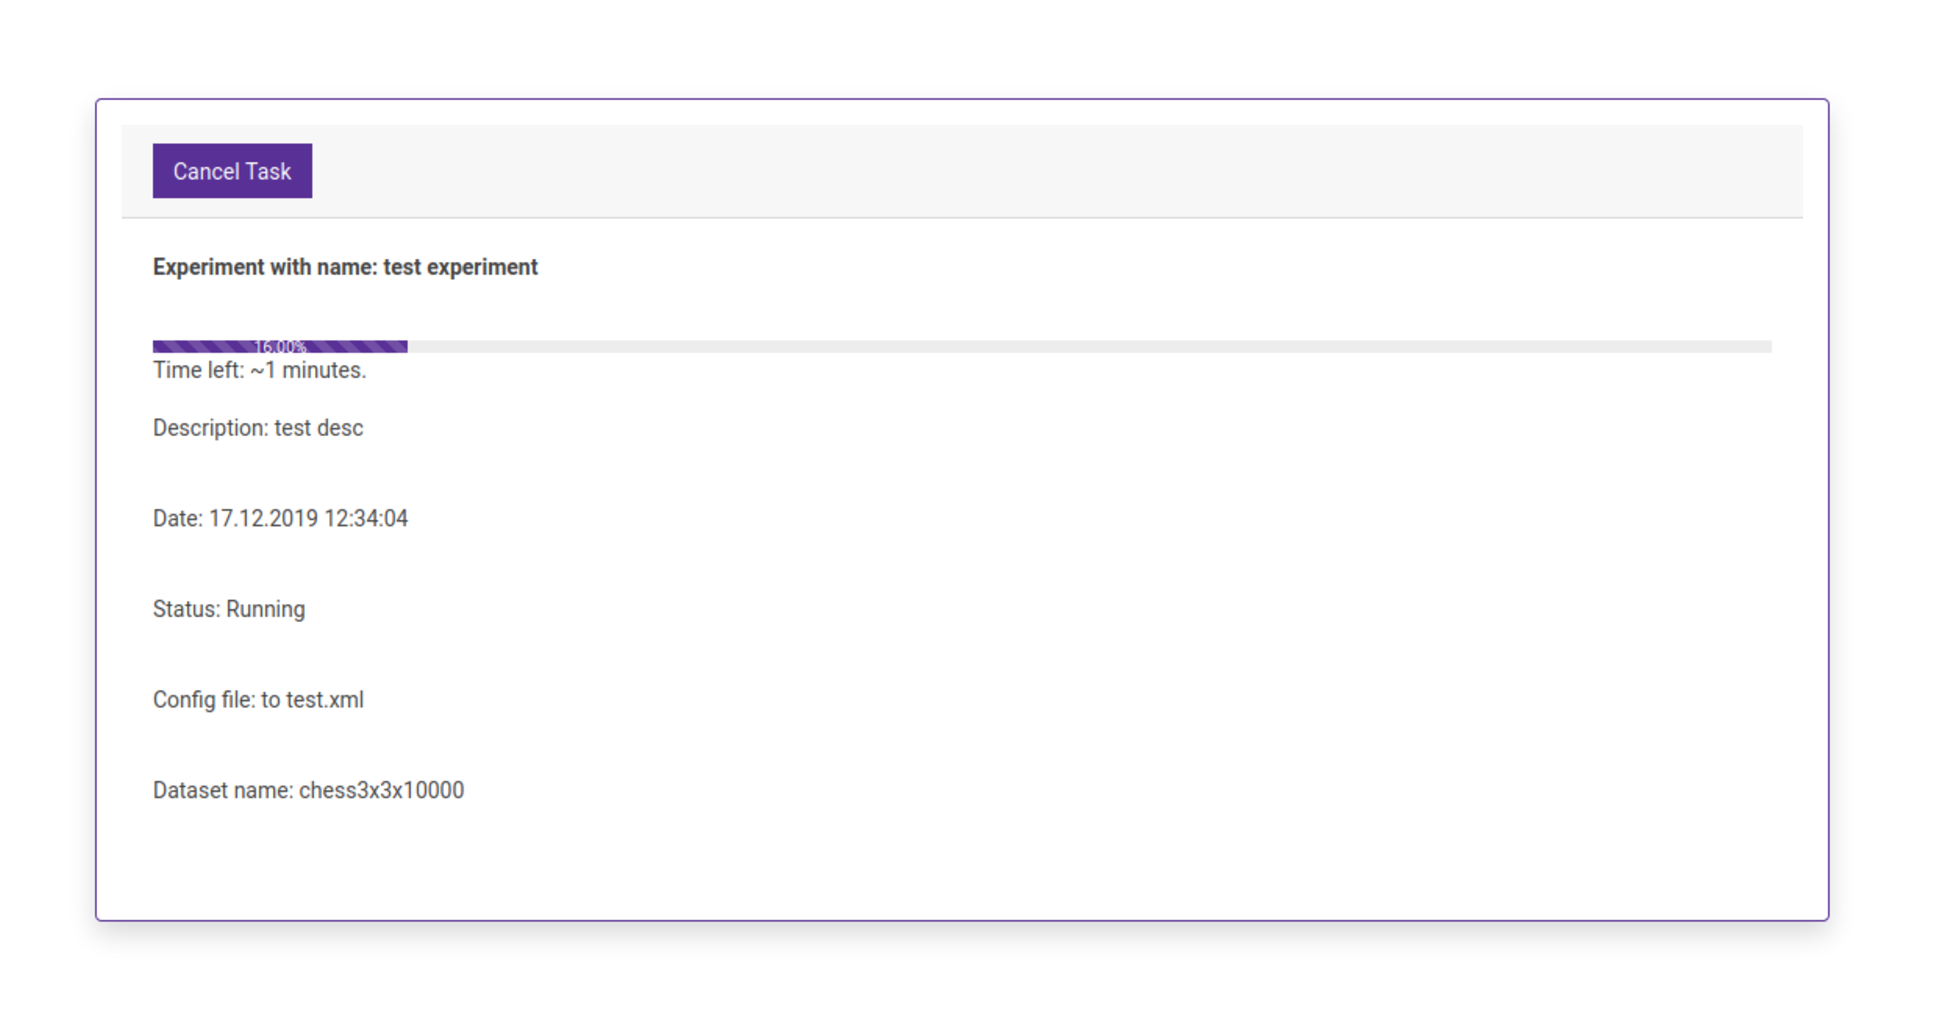
\includegraphics[width=15cm]{grafika/progress_bar.eps}
	\caption{Widok uruchomionego eksperymentu.}
	\label{rys15_progress_bar}
\end{figure}

\begin{figure}[htb]
	\centering
	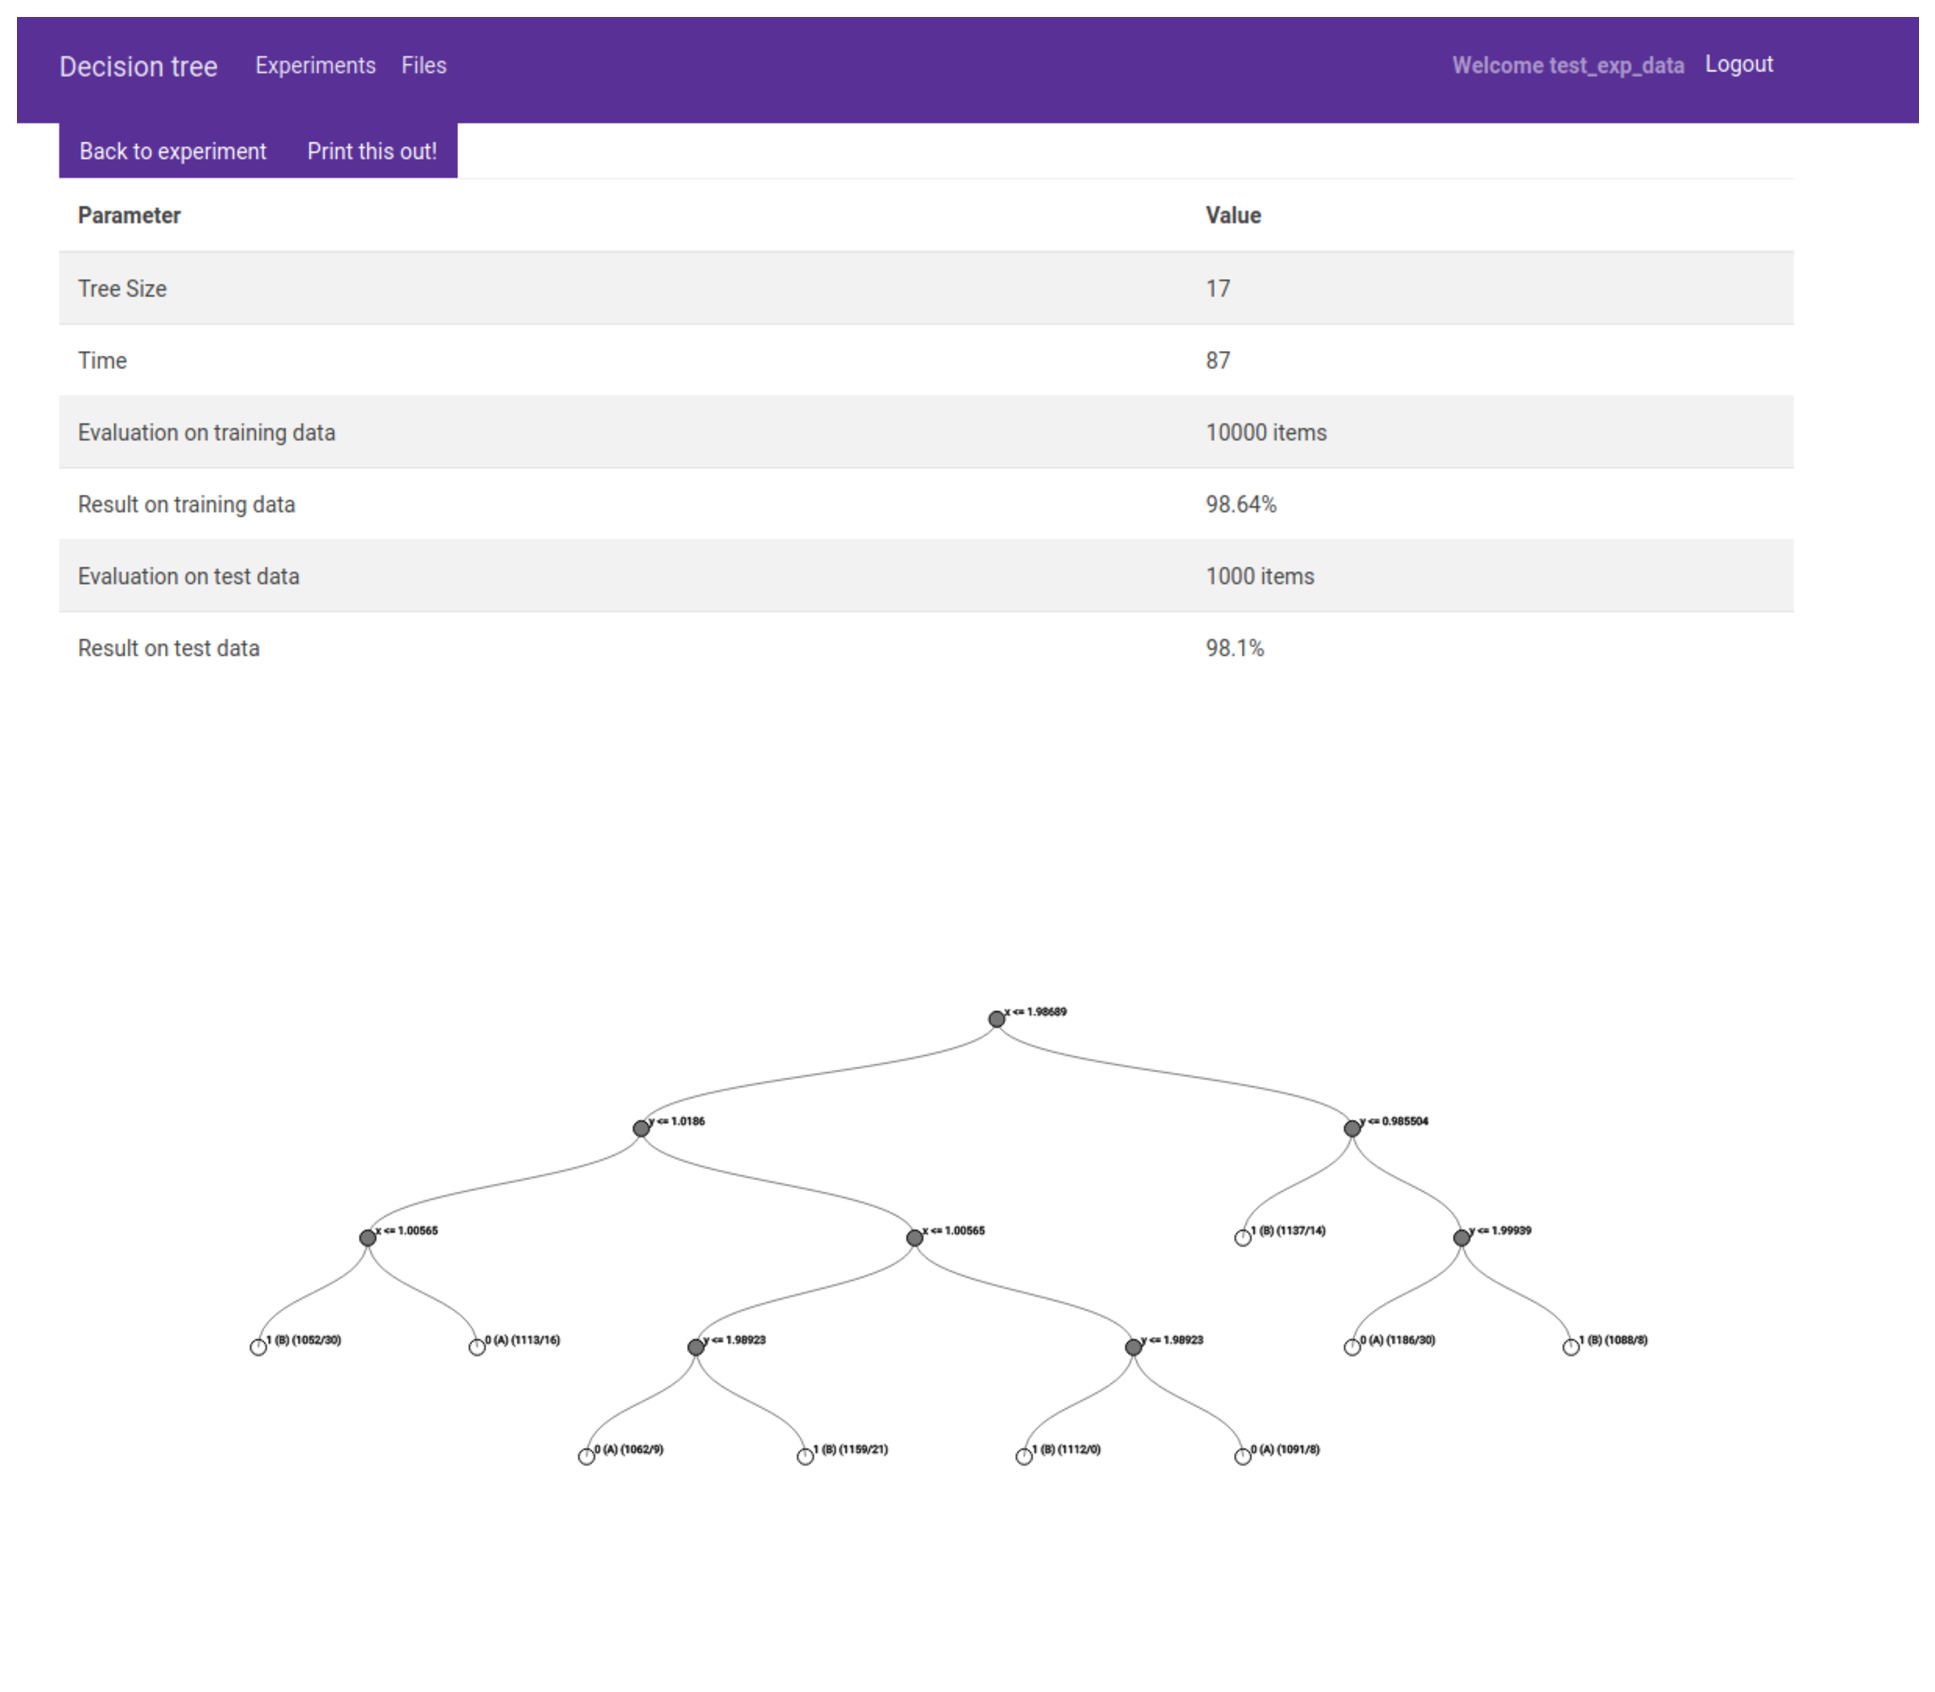
\includegraphics[width=15cm]{grafika/tree_veiw.eps}
	\caption{Widok wyniku eksperymentu.}
	\label{rys16_tree_veiw}
\end{figure}

\begin{figure}[htb]
	\centering
	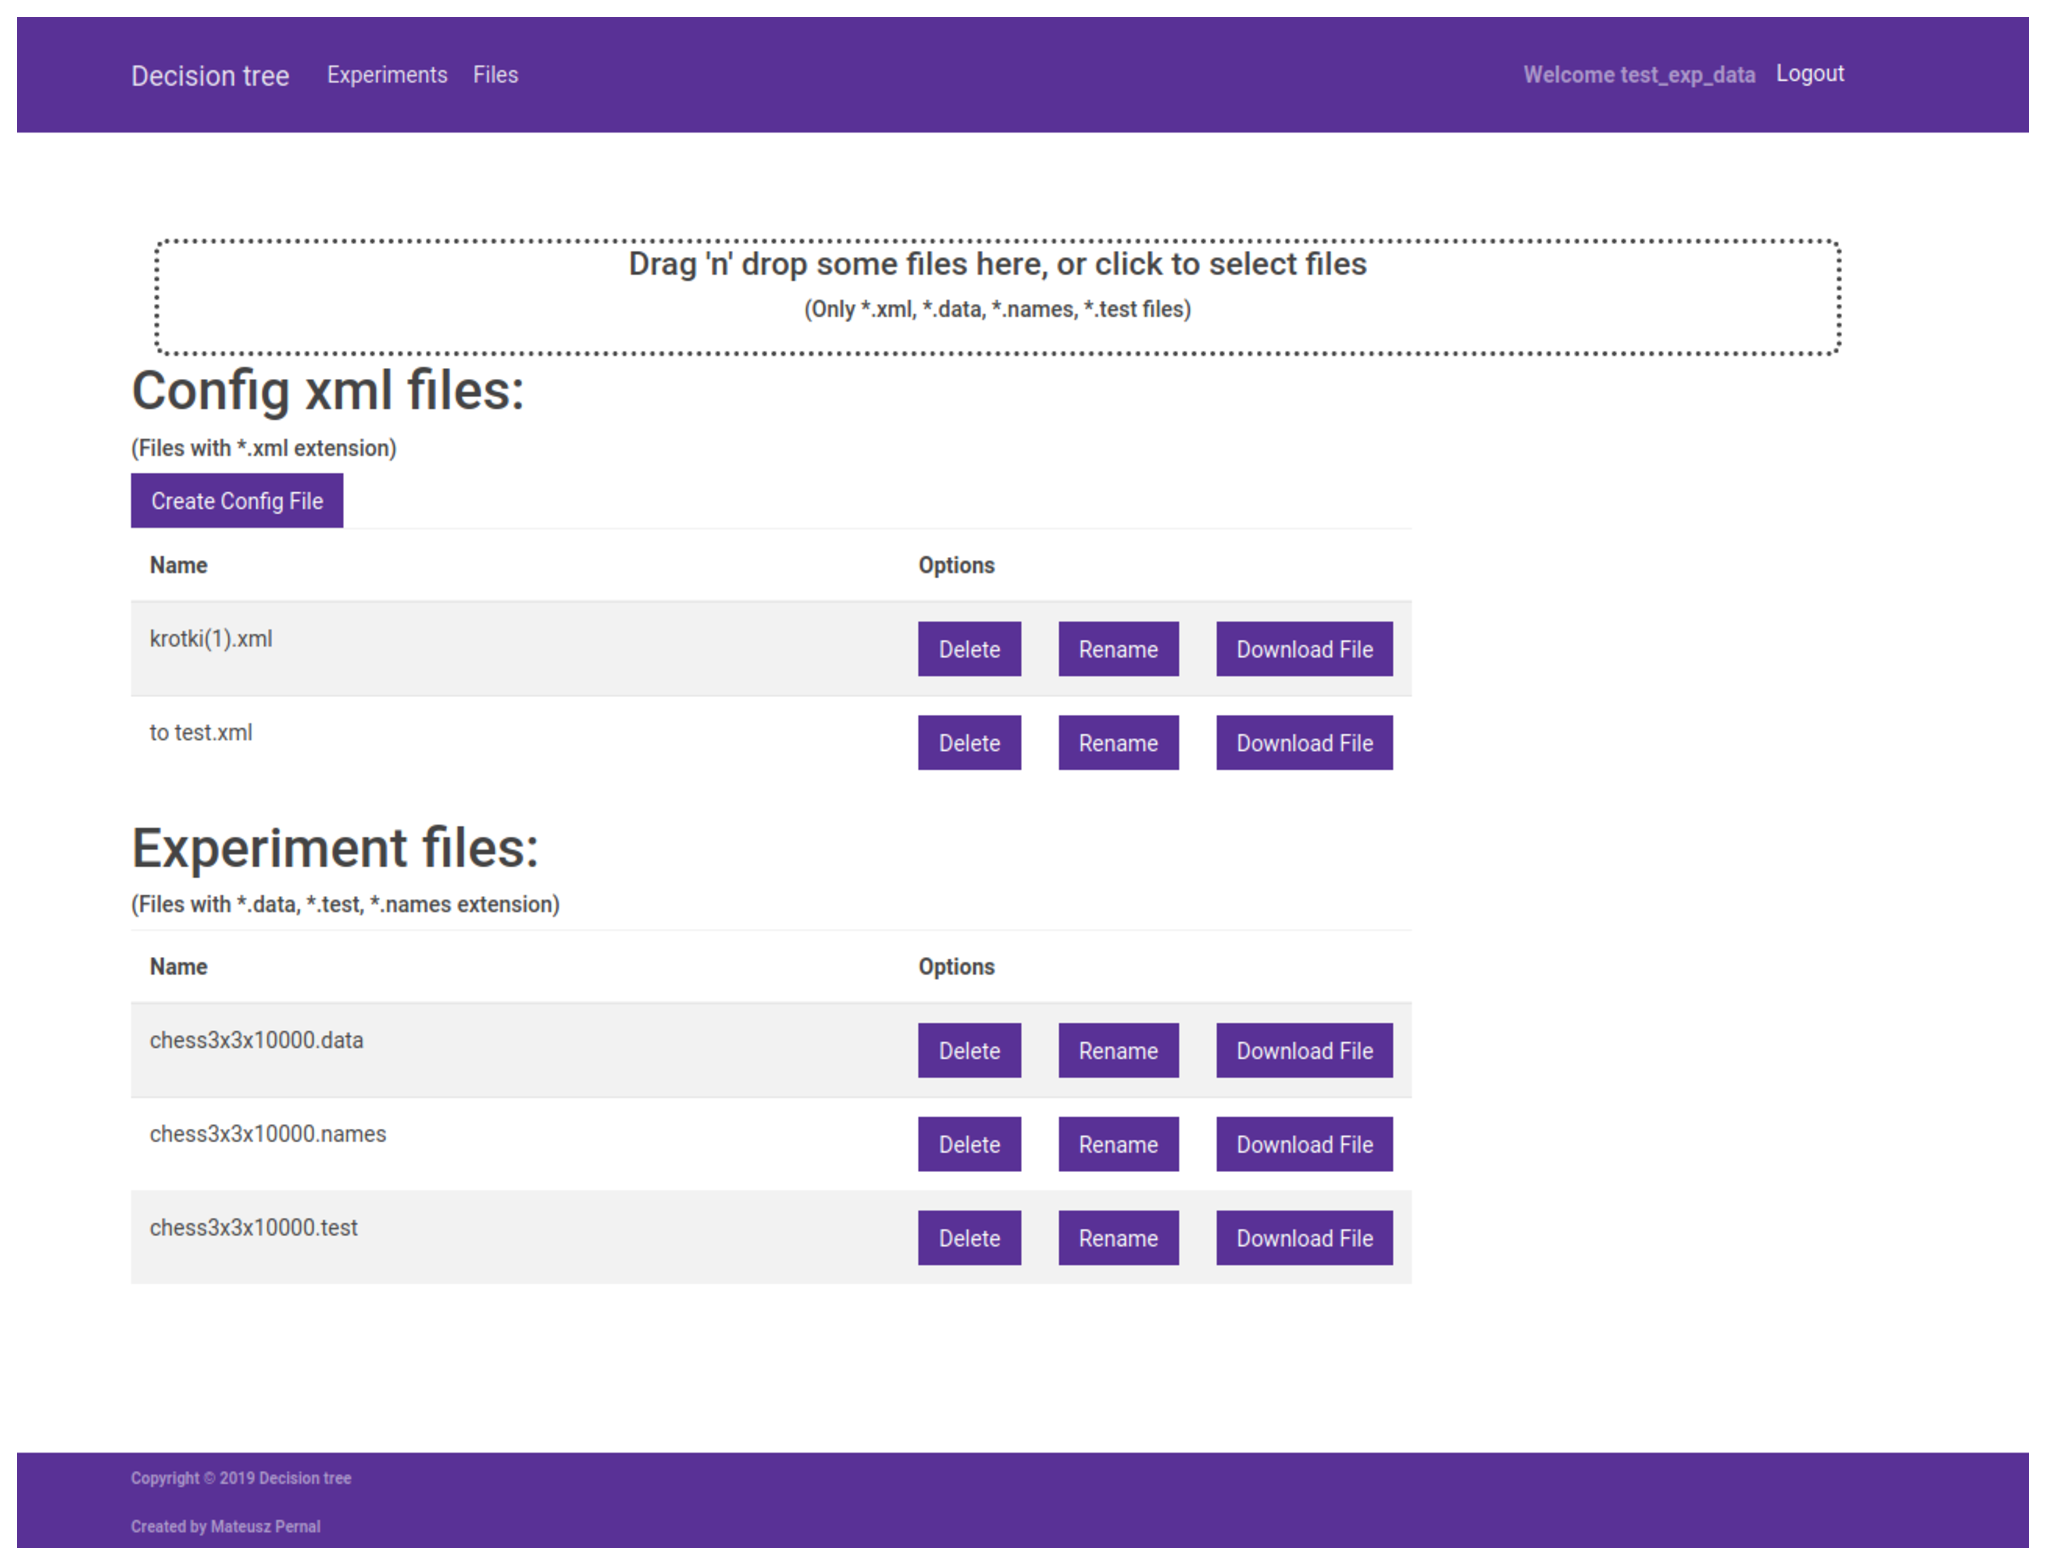
\includegraphics[width=15cm]{grafika/file_page.eps}
	\caption{Widok strony do zarządzania plikami.}
	\label{rys17_file_page}
\end{figure}

\begin{figure}[htb]
	\centering
	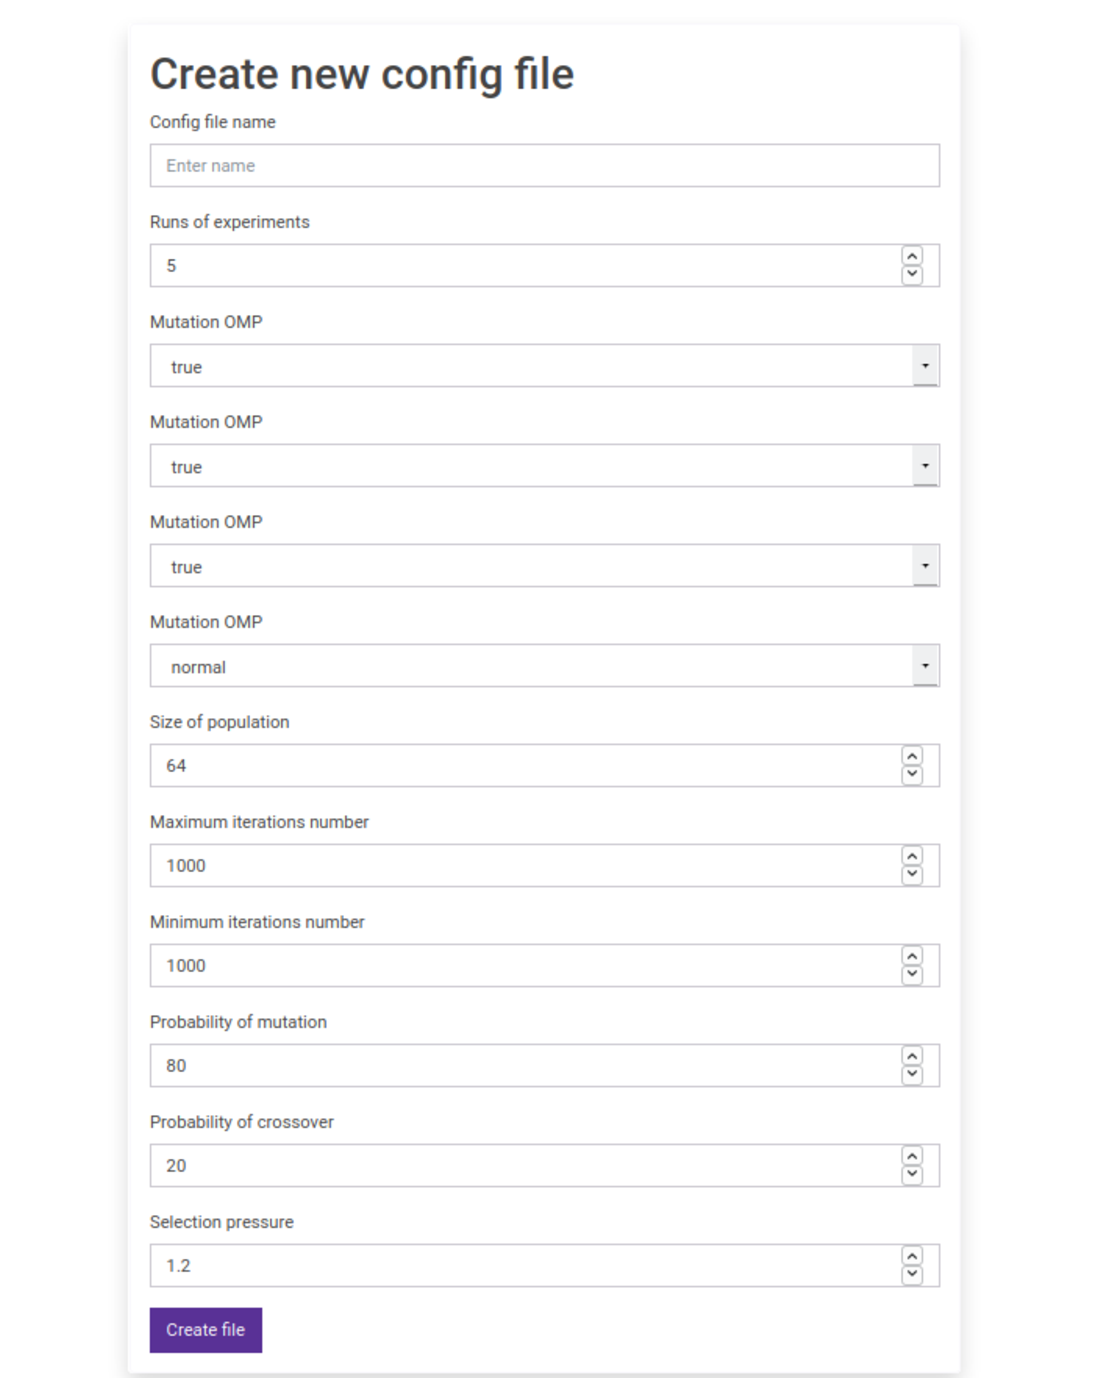
\includegraphics[height=10cm]{grafika/config_form.eps}
	\caption{Formularz tworzenia nowego pliku konfiguracyjnego.}
	\label{rys18_config_form}
\end{figure}

\begin{figure}[htb]
	\centering
	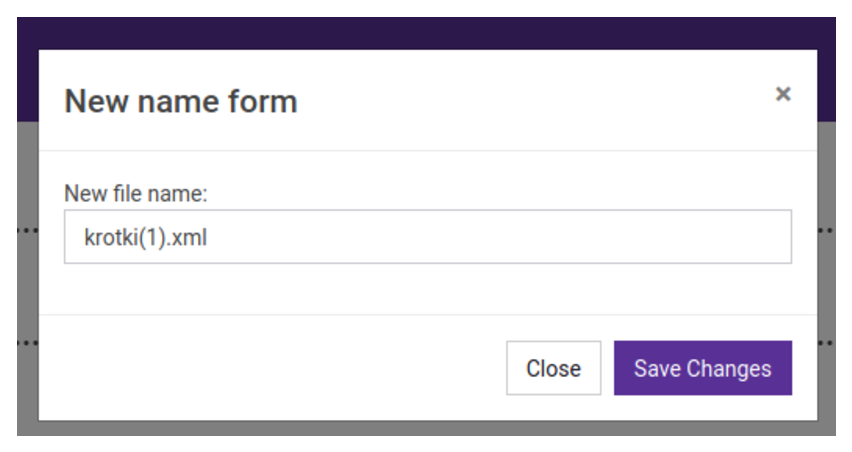
\includegraphics[width=9cm]{grafika/edit_name.eps}
	\caption{Formularz edycji nazwy pliku.}
	\label{rys19_edit_name}
\end{figure}

Użytkownik może wykonywać dodatkowe operacje po przez panel wyświetlenia szczegółów doświadczenia. Jedną z nich jest opcja edycji eksperymentu za pomocą formularza (Rys. \ref{rys13_edit_experiment}). Zatwierdzenie zmian jest możliwe tylko wtedy, gdy występuje chociaż jedna zmiana w modelu.  Kolejną funkcjonalnością znajdującą się na pasku akcji stanowi udostępnianie eksperymentu innym osobom. W formularzu wyświetlają się kontrolki do nadawania praw, które zostały przedstawione na Rys. \ref{rys14_share_form}. Eksperyment po udostępnieniu pojawi się na liście wszystkich doświadczeń u drugiej osoby. Natomiast na końcu nazwy w nawiasach zostanie dodana nazwa oryginalnego właściciela. 


\begin{figure}[htb]
	\centering
	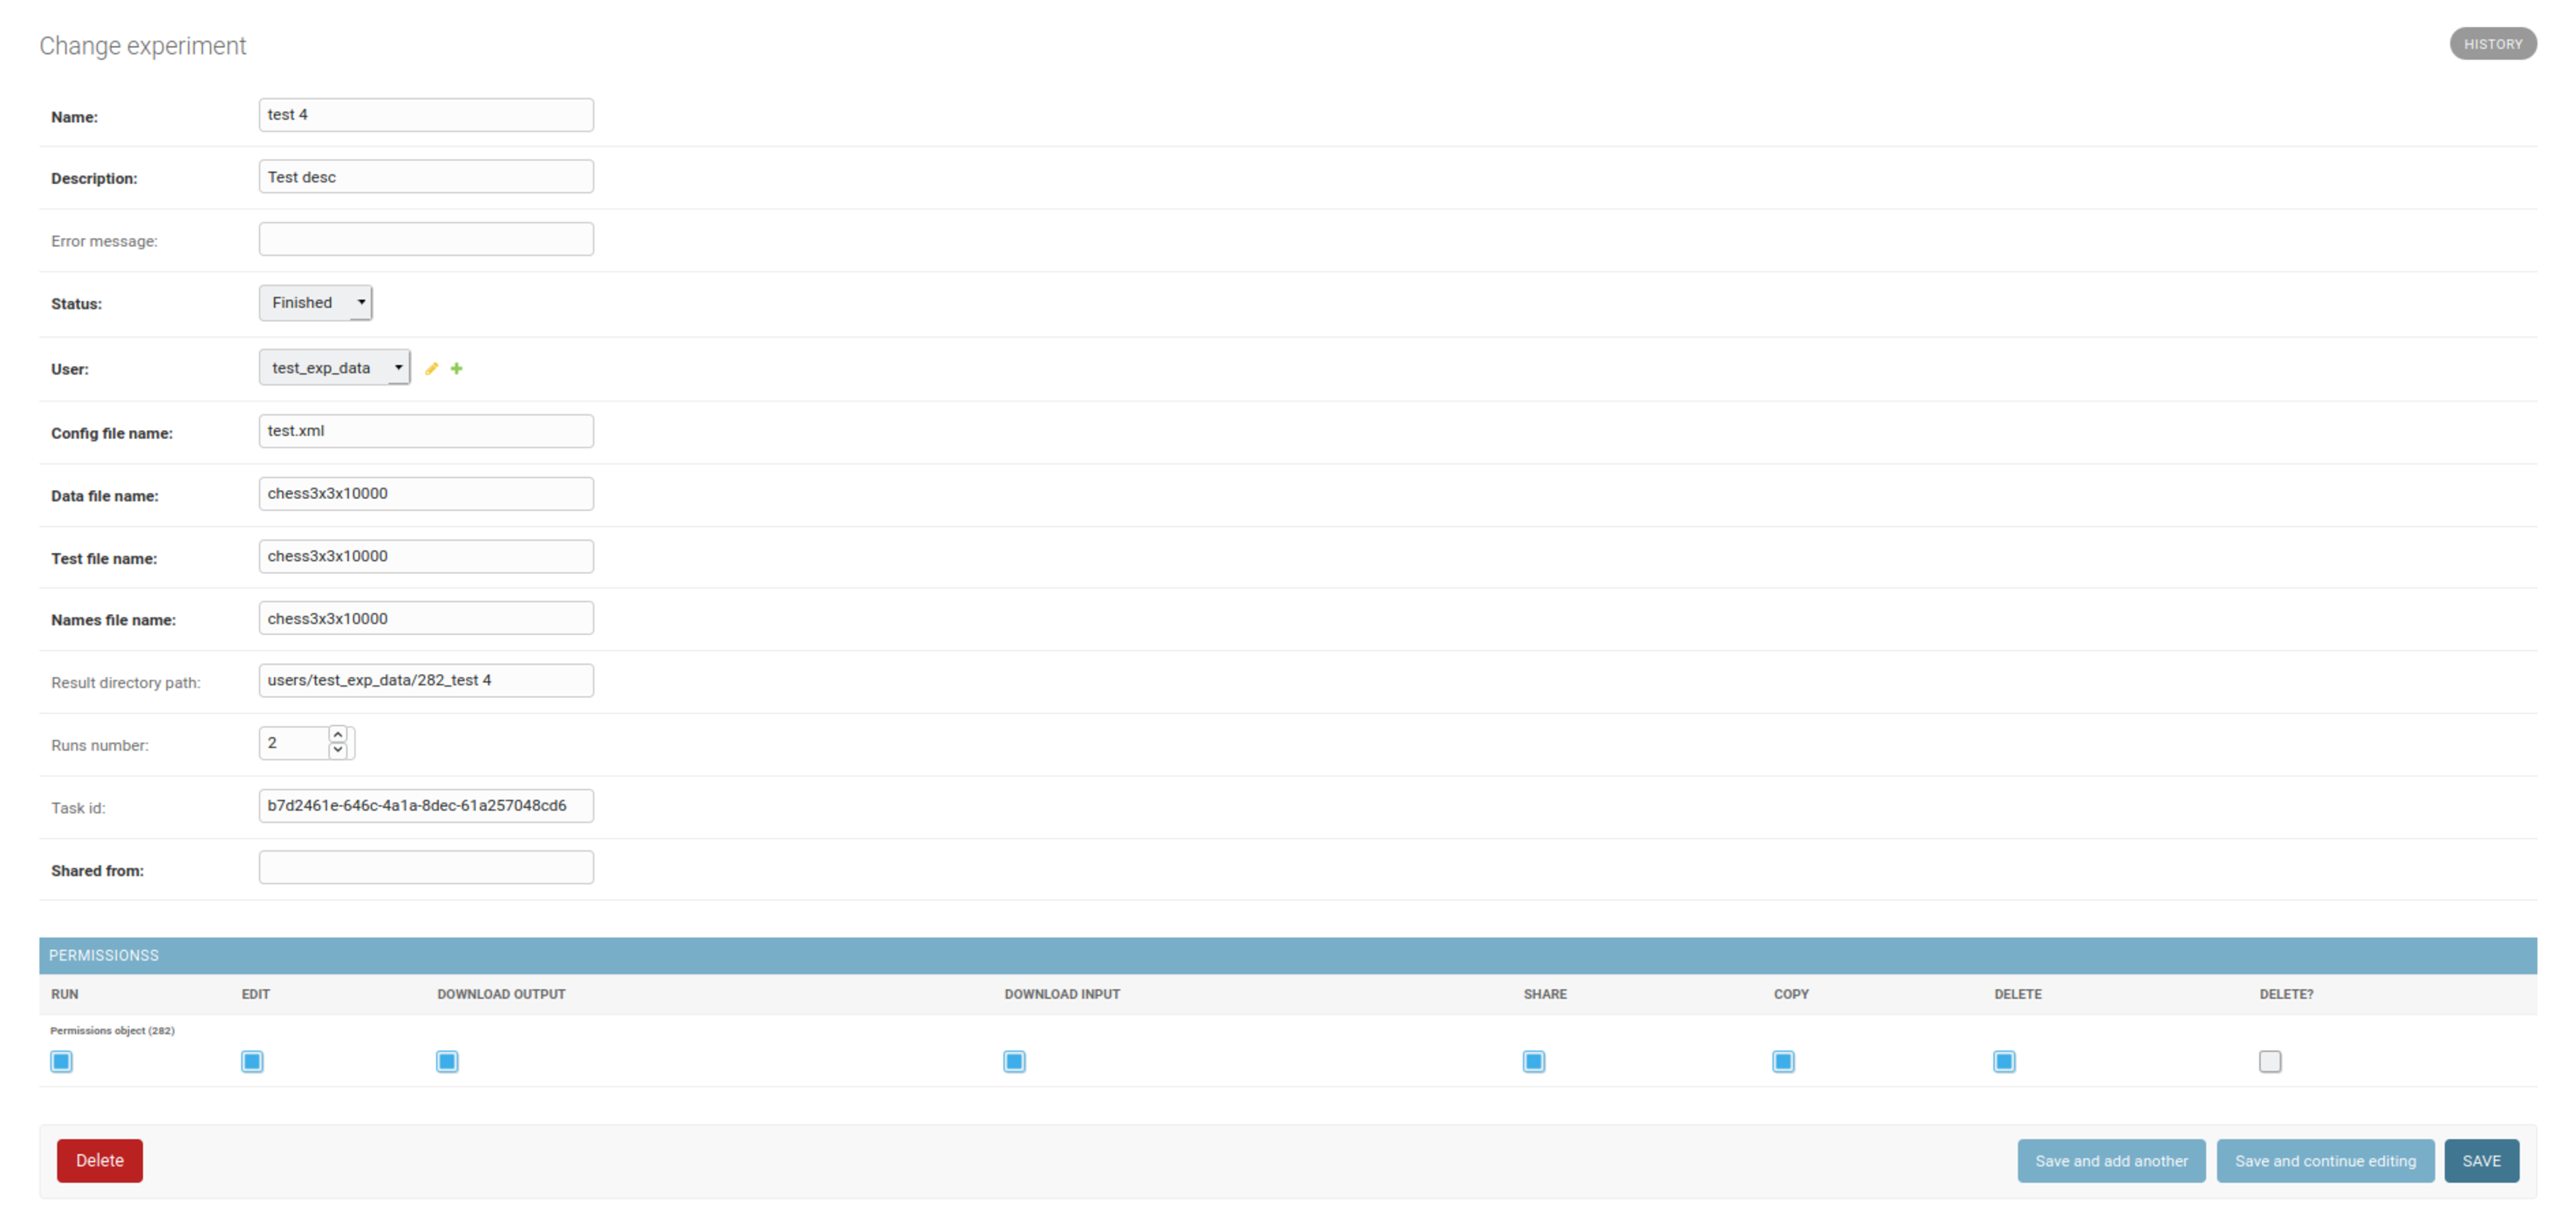
\includegraphics[width=15cm]{grafika/admin_exp.eps}
	\caption{Formularz edycji nazwy pliku.}
	\label{rys20_admin_exp}
\end{figure}

Aplikacja udostępnia również panel administratora dostępny pod adresem \enquote{decisontree.pl\textbackslash{admin}}. Po autoryzacji admin może zarządzać modelami w bazie, ale także zmieniać role użytkowników. Również w dowolnym momencie ma opcje zmiany uprawnień dostępowych do eksperymentu, przez co może ograniczyć lub nadać prawa. Widok zarządzania eksperymentem został przedstawiony na Rys. \ref{rys20_admin_exp}.





\section{Testy aplikacji}